\chapter{Evaluation and Discussion} \label{chap:results}

\minitoc

The assessment of generative \ac{AI} models for audio is pivotal in advancing the field of audio generation and synthesis. It is imperative to comprehend the capabilities and limitations of these models for their effective development and implementation. This chapter presents the outcomes and analysis of experiments performed with the GANmix architecture, utilizing objective metrics based on loss functions. The aim of this study is to assess the efficacy of generative \ac{AI} models in producing audio, and to draw insights from their performance.

The experiments were conducted utilizing different hardware configurations, For \acp{GPU}, it consisted of Kaggle's Tesla V100, \ac{LIACC}'s GeForce GTX 1080, and \ac{LIACC}'s GPU Quadro RTX 8000. These configurations, along with the utilization of the PyTorch deep learning framework, allowed for proficient training and assessment of the generative \ac{AI} models.

In this chapter, the author describes the experimental setup in Section~\ref{sec:res-setup}, comprising both hardware and software configurations, alongside the GANmix architecture. The experiments' outcomes are presented in Section~\ref{sec:res-presentation} with line plots exhibiting the generator and discriminator's loss evolution per epoch. Additionally, the resulting spectrograms are presented to offer a graphical depiction of the produced audio.

Following the presentation of results, the author analyzes and interprets the findings in Section~\ref{sec:res-analysis}, identifying trends, patterns, and significant insights that emerged from the experiments. Comparisons are conducted among various models and variations in the GANmix framework for evaluating their respective performances.

Furthermore, in Section~\ref{sec:limitations}, the author addresses any limitations or challenges encountered during the evaluation process. These factors may include hardware limitations or other constraints that impact the performance of the models.

\section{Experimental Setup} \label{sec:res-setup}

This section outlines the experimental setup utilized to assess the audio generation capabilities of the GANmix model.

The GANmix model was trained using the \ac{BCE} loss, which was implemented through pytorch's \texttt{BCEWithLogitsLoss} module. Although \ac{BCE} is commonly employed for binary classification, it can also effectively train the generator in \acp{GAN}. In the context of GANmix, the generator's goal is to create authentic embeddings that can fool the discriminator into classifying them as authentic. To achieve this, the generator's loss is calculated using the discriminator's output for the fake embeddings generated by the generator and the true label --- either real or fake --- for a real embedding.

By using \ac{BCE}, the generator calculates its loss by measuring the difference between the discriminator's classification of genuine and false embeddings. This loss directs the generator to generate more realistic embeddings over time by minimizing this difference. Therefore, despite being a binary classification loss function, \ac{BCE} is a suitable approach for training the generator in \acp{GAN}.

Two datasets, the Audio MNIST dataset~\cite{becker_interpreting_2018} and the Clotho dataset~\cite{drossos_clotho_2019}, were utilized in these experiments. These datasets were previously described in detail in Section~\ref{sec:sol-datasets}.

The Audio MNIST dataset contains short audio clips where each clip represents a spoken digit. This dataset sets a standard for evaluating audio classification tasks.

In contrast, the Clotho dataset is more extensive and diverse. It offers a variety of audio samples including environmental sounds and speech from various sources. This dataset offers a diverse and comprehensive range of audio data, allowing the GANmix model to learn and generate audio samples that capture the complexity and diversity present in real-world audio recordings.

For a thorough understanding of the datasets, including their characteristics, preprocessing steps, and data augmentation techniques, please refer to Section~\ref{sec:sol-datasets}.

The experiments were conducted on three distinct hardware configurations, referred to as \textit{Kaggle}, \textit{\ac{LIACC} 1}, and \textit{\ac{LIACC} 2}, each selected based on the available resources during the development process.

Kaggle, the initial configuration implemented for the GANmix model development phase, utilized a Tesla V100 \ac{GPU} equipped with 12 \ac{GB} of memory, 73.1 \ac{GB} of disk space, and 13 \ac{GB} of \ac{RAM}.

As development progressed, the \ac{LIACC} 1 became available, which offered around the same computational power, \ac{LIACC} 1 used a GeForce GTX 1080 \ac{GPU} with 8 \ac{GB} of memory, 50 \ac{GB} of disk space, and 32 \ac{GB} of \ac{RAM}.

In the final stages of the project, the third configuration, \ac{LIACC} 2, was made available. \ac{LIACC} 2 employed a \ac{GPU} Quadro RTX 8000 with 48 \ac{GB} of memory, 50 \ac{GB} of disk space, and 128 \ac{GB} of \ac{RAM}, allowing for extensive training and evaluation of the GANmix model.

These hardware configurations were chosen to facilitate GANmix model training and evaluation throughout the developmental stages.

The GANmix model was implemented using the Python programming language and the PyTorch deep learning framework. There is a further discussion about this framework in Section~\ref{sec:dl-frameworks}.

Before training, a preprocessing step was applied to the audio data by randomly cropping the dataset sample to the duration of 5 seconds. Random cropping is discussed further in Section~\ref{sec:findings}. This approach enabled a more diverse dataset since the majority of its samples had longer durations. Random cropping aided in capturing diverse segments of the audio and improved the model's ability to generate realistic audio samples.

The GANmix model underwent training using a set of specific hyperparameters. The batch size ranged between 1 and 32, providing varying trade-offs between computational efficiency and model convergence. The training epochs varied from a few tens to a few hundreds, depending on the dataset and model complexity. 

The learning rates utilized to train the GANmix model ranged from $1 \times 10^{-5}$ to $1 \times 10^{-2}$.

The training process was stopped based on evidence of convergence before reaching any predetermined number of epochs. This choice was made to optimize computational resources while still obtaining satisfactory results. In the analysis presented in section~\ref{sec:res-presentation}, the graphs are set to plot a maximum of 100 epochs.
\documentclass{beamer}

% DELETE THE NEXT LINE FOR THE PRESENTATION
\setbeameroption{show notes on second screen=right}

\usetheme{MyTheme}

\usepackage{graphicx}
\usepackage{biblatex}

\addbibresource{sections/references.bib}

\title{Synthesizing Audio from Textual Input}
\subtitle{Development and Comparison of Generative AI Models}
\author{Márcio Duarte \\
    \and Luís Paulo Reis (Supervisor) \\
    \and Gilberto Bernardes (Second Supervisor)
}
\institute{Faculdade de Engenharia da Universidade do Porto}
% TODO: Change date to the date of the presentation
\date{\today}

\begin{document}

\begin{frame}
  \titlepage
\end{frame}

\begin{frame}[t]
  \frametitle{Outline}
  \begin{columns}[T]
    \begin{column}{.5\textwidth}
      \tableofcontents[sections={1-2}]
    \end{column}
    \begin{column}{.5\textwidth}
      \tableofcontents[sections={3-}]
    \end{column}
  \end{columns}
\end{frame}
% Define the introduction
\section{Introduction}

\subsection{Context}

\begin{frame}
    \frametitle{Overview of Computer Science and its Evolution}
    \begin{itemize}
        \item ``Computer Science is the study of computation and information.''~\cite{university_of_york_what_nodate}
        \item Evolution of Computer Science: From traditional programming to advanced Machine Learning (ML) and Deep Learning (DL) techniques.
        \item Importance of Big Data and Parallel Computing: Catalysts for advancements in ML and DL.
        \item Role of Deep Learning: Automated feature extraction, particularly effective in tasks like image and audio processing.
        \item Significance of Generative Models: Creating synthetic data for various applications.
    \end{itemize}
\end{frame}

\begin{frame}
    \frametitle{Timeline of Key Events in AI and Machine Learning}
    \begin{enumerate}
        \item \textbf{1958 - Birth of Modern AI:}
              \begin{itemize}
                  \item F. Rosenblatt proposes three fundamental questions leading to the development of the perceptron.
              \end{itemize}

        \item \textbf{1960s - Perceptron Convergence:}
              \begin{itemize}
                  \item Intensive work on convergence algorithms for the perceptron.
              \end{itemize}

        \item \textbf{1969 - Limitations of Perceptrons:}
              \begin{itemize}
                  \item Minksy and Papert demonstrate the limitations of perceptrons, leading to a slowdown in AI research.
              \end{itemize}

        \item \textbf{1980s - Emergence of Multilayer Neural Networks:}
              \begin{itemize}
                  \item Studies on learning under multilayer neural networks.
              \end{itemize}

        \item \textbf{1986 - Backpropagation:}
              \begin{itemize}
                  \item Rumelhart et al. describe backpropagation, a key learning procedure for neural networks.
              \end{itemize}

        \item \textbf{1990s - Second Winter of AI:}
              \begin{itemize}
                  \item Decreased investments in ML due to lack of real successes.
              \end{itemize}

        \item \textbf{Turn of the Millennium - Resurgence of ML:}
              \begin{itemize}
                  \item Emergence of three trends: Big Data, reduced cost of parallel computing, and interest in Deep Neural Networks (DNN).
              \end{itemize}

        \item \textbf{2010s - DL in Everyday Applications:}
              \begin{itemize}
                  \item DL becomes integral for various computer-made tasks, including text translation, recommender systems, and more.
              \end{itemize}

        \item \textbf{Generative Models and Their Impact:}
              \begin{itemize}
                  \item Introduction of generative models and their applications in image and text generation.
              \end{itemize}

        \item \textbf{2020s - Decade of Generative Applications:}
              \begin{itemize}
                  \item Rise of generative
              \end{itemize}
    \end{enumerate}
\end{frame}


\subsection{Background}

\begin{frame}
    \frametitle{Introduction to Background}
    % Briefly introduce the vast body of research on Deep Learning (DL).
\end{frame}

\begin{frame}
    \frametitle{Digital Audio Processing}
    % Explain how audio is represented digitally and how it can be processed.
\end{frame}

\begin{frame}
    \frametitle{Foundations for Enhancing Generative Models for Audio}
\end{frame}

\begin{frame}
    \frametitle{Deep Learning Frameworks}
\end{frame}

\begin{frame}
    \frametitle{State of the Art Generative Models}
\end{frame}

\subsection{Motivation}
% Explain what motivated you to conduct this research. What personal or professional experiences inspired your work?
% You can also use this slide to discuss your research goals. What did you hope to achieve by conducting this research?

\begin{frame}{Motivation}
    \begin{enumerate}
        \item \textbf{ML in Audio Processing}
              \begin{itemize}
                  \item ML techniques enhance sound synthesis, restoration, and speech recognition.
                  \item Learn complex patterns, improving quality and efficiency.
              \end{itemize}
        \item \textbf{Revolutionizing Sound Generation}
              \begin{itemize}
                  \item Integration of ML transforms sound creation and experience.
                  \item Opens creative avenues for artists, impacts industries like film, gaming, VR.
              \end{itemize}
        \item \textbf{Need for Further Research}
              \begin{itemize}
                  \item Urgency for studies in sound generation technologies.
                  \item This dissertation contributes significantly, offering resources for exploration.
              \end{itemize}
        \item \textbf{Impact and Contribution}
              \begin{itemize}
                  \item Reshaping human potential in sound creation through digital technologies.
                  \item Valuable resource for audio processing professionals, guiding future endeavors.
              \end{itemize}
        \item \textbf{Overall Significance}
              \begin{itemize}
                  \item Valuable contribution to audio processing and machine learning field.
              \end{itemize}
    \end{enumerate}
\end{frame}

\subsection{Research objectives}

\begin{frame}{Research Objectives}
    \begin{enumerate}
        \item Make a study of the current state-of-the-art deep learning architectures, focusing on generative ones.
        \item Examine prior algorithms that can process sound for augmentation, feature extraction, or other purposes.
        \item Make a study of the current state-of-the-art architectures used to develop sounds artificially.
        \item Develop end-to-end systems that can synthesize sound from any given text input, while accounting for hardware constraints and ensuring reliable performance.
        \item Evaluate the systems’ ability to generate a sound from the given textual input accurately.
    \end{enumerate}
\end{frame}
\section{State of the Art}

\subsection{Introduction}
\begin{frame}
    \frametitle{State of the Art}
    \begin{itemize}
        \item There are different types of sound generation methods, depending on the level of abstraction and supervision involved
        \item Four types of sound generation methods are considered in this thesis:
              \begin{itemize}
                  \item Traditional
                  \item Unsupervised
                  \item Vocoders
                  \item End-to-end models
              \end{itemize}
    \end{itemize}
\end{frame}

\subsection{Traditional Soundscape Generation}

\begin{frame}
    \frametitle{Traditional Soundscape Generation}

    \textbf{Notable Tools}
    \begin{itemize}
        \item \textit{Scaper}~\cite{salamon_scaper_2017}: Open-source library for synthetic sound environments
        \item SEED~\cite{bernardes_seed_2016}: System for resynthesizing environmental sounds with precise control over variation
        \item Physics-Based Concatenative Sound Synthesis~\cite{magalhaes_physics-based_2020}: Creates novel auditory experiences by assembling pre-existing sound segments
    \end{itemize}
\end{frame}

\subsection{Unsupervised Sound Generation}

\begin{frame}
    \frametitle{Unsupervised Sound Generation}

    \textbf{Approach}
    \begin{itemize}
        \item Learn sound features and distributions without explicit labels
        \item Utilize unlabeled audio data for pattern capture and structure learning
        \item Valuable when labeled datasets are limited or costly
    \end{itemize}

    \textbf{Notable Models}
    \begin{itemize}
        \item WaveGAN~\cite{donahue_adversarial_2019}: Unsupervised waveform synthesis using modified GAN
        \item Generative Transformer~\cite{verma_generative_2021}: Autoregressive prediction of audio samples using transformer networks
        \item wav2vec 2.0~\cite{baevski_wav2vec_2020}: Speech generation model with convolutional feature encoder, Transformer, and quantization module
        \item SoundStream~\cite{zeghidour_soundstream_2021}: Neural audio codec for efficient audio compression
    \end{itemize}
\end{frame}


\subsection{Vocoders}

\begin{frame}
    \frametitle{Vocoders}

    \textbf{Notable Models}
    \begin{itemize}
        \item WaveNet~\cite{oord_wavenet_2016}: Generative neural network using dilated causal convolutions for raw audio waveform generation
        \item WaveNet Variants: Models like WaveRNN, FloWaveNet, and Fast WaveNet reduce complexity while maintaining effectiveness
        \item MelGAN~\cite{kumar_melgan_2019}: GAN-based model using Mel-Spectrograms for coherent audio waveform generation
        \item GANSynth~\cite{engel_gansynth_2019}: GAN using log-magnitude spectrograms and phases for waveform generation
        \item HiFi-GAN~\cite{kong_hifi-gan_2020}: GAN model combining efficiency and high-fidelity speech synthesis
    \end{itemize}
\end{frame}


\subsection{End-to-End Models}


\begin{frame}[allowframebreaks]
    \frametitle{End-to-End Audio Models Comparison}

    \begin{table}[ht]
        \centering
        \caption{A comparison of different end-to-end generative models for audio.}
        \begin{tabularx}{\textwidth}{|X|l|X|X|}
            \hline
            \textbf{Model}                           & \textbf{Type} & \textbf{Input}            & \textbf{Output}                        \\ \hline
            Char2wav~\cite{sotelo_char2wav_2017}     & Speech        & Text prompt               & Raw audio waveform                     \\ \hline
            VALL-E~\cite{wang_neural_2023}           & Speech        & Text and acoustic prompt  & Raw audio waveform                     \\ \hline
            Jukebox~\cite{dhariwal_jukebox_2020}     & Music         & Genre, artist, and lyrics & Raw audio waveform                     \\ \hline
            Riffusion~\cite{forsgren_riffusion_2022} & Music         & Text prompt               & Raw audio waveform                     \\ \hline
            MusicLM~\cite{agostinelli_musiclm_2023}  & Music         & Text prompt               & Raw audio waveform                     \\ \hline
            SampleRNN~\cite{mehri_samplernn_2017}    & General       & None                      & Raw audio waveform                     \\ \hline
            AudioLM~\cite{borsos_audiolm_2022}       & General       & Text prompt               & Raw audio waveform                     \\ \hline
            DiffSound~\cite{yang_diffsound_2022}     & General       & Text prompt               & Mel-spectrogram and raw audio waveform \\ \hline
            AudioGen~\cite{kreuk_audiogen_2023}      & General       & Text prompt               & Mel-spectrogram and raw audio waveform \\ \hline
        \end{tabularx}
        \label{tab:end-to-end-audio-models}
    \end{table}
\end{frame}

\begin{frame}
    \frametitle{Text-to-Speech (TTS)}

    \textbf{Definition}
    \begin{itemize}
        \item Convert written text into synthesized speech
        \item Use deep neural networks for direct mapping
        \item Notable TTS Models:
              \begin{itemize}
                  \item Char2wav
                  \item VALL-E
              \end{itemize}
    \end{itemize}
\end{frame}

\begin{frame}
    \frametitle{Generative Music}

    \textbf{Definition}
    \begin{itemize}
        \item Create music using generative techniques
        \item End-to-end models for composing new musical pieces
        \item Notable Generative Music Models:
              \begin{itemize}
                  \item Jukebox
                  \item Riffusion
                  \item MusicLM
              \end{itemize}
    \end{itemize}

\end{frame}

\begin{frame}
    \frametitle{General Text-to-Audio}

    \textbf{Definition}
    \begin{itemize}
        \item Convert various forms of text to corresponding audio outputs
        \item Applications: sound effects, voice transformation, environmental sound synthesis
        \item Notable Text-to-Audio Models:
              \begin{itemize}
                  \item SampleRNN
                  \item AudioLM
                  \item DiffSound
                  \item AudioGen
              \end{itemize}
    \end{itemize}

\end{frame}


\subsection{AudioLM}
\begin{frame}{AudioLM}
    \begin{itemize}
        \item A framework for high-quality audio generation with long-term consistency~\cite{borsos_audiolm_2022}.
        \item Maps input audio to a sequence of discrete tokens and treats audio generation as a language modeling task.
        \item Achieves high-quality synthesis and long-term structure through a hybrid tokenization scheme of semantic and acoustic tokens.
        \item Consists of three main components: tokenizer, language model, and detokenizer.
        \item Generates syntactically and semantically plausible speech and music continuations without any transcript or annotation.
    \end{itemize}
\end{frame}

\subsection{DiffSound}

\begin{frame}{DiffSound}
    \begin{itemize}
        \item A novel text-to-sound generation framework that uses a text encoder, a VQ-VAE, a decoder, and a vocoder~\cite{yang_diffsound_2022}.
        \item Takes text as input and outputs synthesized audio corresponding to the input text.
        \item Uses a diffusion decoder (DiffSound) that predicts and refines all Mel-Spectrogram tokens in one step, resulting in better and faster generation than an AR decoder.
        \item Produces high-quality sound synthesis for various domains such as speech, music, and environmental sounds.
    \end{itemize}
\end{frame}


\subsection{AudioGen}
\begin{frame}{AudioGen}
    \begin{itemize}
        \item An auto-regressive generative model that generates audio samples conditioned on text inputs~\cite{kreuk_audiogen_2023}.
        \item Learns a discrete representation of the raw audio using an AE method and trains a Transformer language model over the learned codes, conditioned on textual features.
        \item Uses an augmentation technique that mixes different audio samples to train the model to separate multiple sources internally.
        \item Explores the use of multi-stream modeling for faster inference, allowing the use of shorter sequences while maintaining a similar bitrate and perceptual quality.
        \item Outperforms evaluated baselines over both objective and subjective metrics and extends to conditional and unconditional audio continuation.
    \end{itemize}
\end{frame}

\section{Development}

\subsection{Datasets}

\begin{frame}
    \frametitle{Dataset Introduction}

    \begin{itemize}
        \item Datasets form the foundation for generative models
        \item Learning material for DL algorithms and evaluation of audio outputs
        \item Two types of datasets: categorical and descriptive
    \end{itemize}

\end{frame}

\begin{frame}
    \frametitle{Table of Datasets}

    \begin{table}[ht]
        \centering
        \caption{Comparison of datasets for soundscapes}
        \label{tab:datasets}
        \begin{tabularx}{\textwidth}{|X|X|X|X|X|}
            \hline
            \textbf{Name}                                           &
            \textbf{Type}                                           &
            \textbf{\# Samples}                                     &
            \textbf{Duration}                                       &
            \textbf{Labels}                                           \\ \hline

            Acoustic Event Dataset \cite{takahashi_deep_2016}       &
            Categorical labeled                                     &
            5223                                                    &
            Average 8.8s                                            &
            One of 28 labels                                          \\ \hline

            AudioCaps \cite{kim_audiocaps_2019}                     &
            Descriptive labeled                                     &
            39597                                                   &
            10s each                                                &
            9 words per caption                                       \\ \hline

            AudioSet \cite{gemmeke_audio_2017}                      &
            Categorical labeled                                     &
            2084320                                                 &
            Average 10s                                             &
            One or more of 527 labels                                 \\ \hline

            Audio MNIST~\cite{becker_interpreting_2018}             &
            Categorical labeled                                     &
            30000                                                   &
            Average 0.6s                                            &
            One of 10 labels                                          \\ \hline

            Clotho \cite{drossos_clotho_2019}                       &
            Descriptive labeled                                     &
            4981                                                    &
            15 to 30s                                               &
            24 905 captions (5 per audio). 8 to 20 words long each    \\ \hline

            FSDKaggle2018 \cite{fonseca_general-purpose_2018}       &
            Categorical labeled                                     &
            11073                                                   &
            From 300ms to 30s                                       &
            One or more of 41 labels                                  \\ \hline

            UrbanSound8K \cite{salamon_dataset_2014}                &
            Categorical labeled                                     &
            8732                                                    &
            Less or equal to 4s                                     &
            One of 10 labels                                          \\ \hline

            YouTube-8M Segments \cite{abu-el-haija_youtube-8m_2016} &
            Categorical labeled                                     &
            237000                                                  &
            5s                                                      &
            One or more of 1000 labels                                \\ \hline
        \end{tabularx}
    \end{table}
\end{frame}


\subsection{Exploratory Experiments}

\begin{frame}
    \frametitle{Exploratory Experiments}
    
    \begin{itemize}
        \item Objective: Gain insights for GANmix development
        \item Experiments: Classification, GAN, AE, VAE
        \item Findings: Foundation for audio representation, GAN effectiveness, AE/VAE capabilities
        \item Impact: Crucial for robust audio generation with GANmix
    \end{itemize}

\end{frame}

\subsection{GANmix}

\begin{frame}
    \frametitle{GANmix: Introduction}

    \begin{itemize}
        \item GANmix: Fusion of GAN and VAE for audio generation under constraints.
        \item Addresses computational limitations for high-quality audio.
        \item Combines GAN's generative power with VAE's latent space manipulation.
    \end{itemize}
\end{frame}

\begin{frame}
    \frametitle{GANmix: Model Architecture}

    \begin{itemize}
        \item Generator and discriminator operate in latent space.
        \item VAE Training: Computational challenge, requires extensive datasets.
        \item AudioLDM's High-Performance: Top model for audio generation.
        \item Accessibility of AudioLDM: Open source, accessible via Hugging Face's model hub.
    \end{itemize}
\end{frame}

\begin{frame}
    \frametitle{GANmix: Experimental Results}

    \begin{itemize}
        \item Preliminary experiments with Audio MNIST: Promising but suboptimal.
        \item Refinements: Different optimizers, model sizes, loss functions.
        \item Clotho dataset: Significant improvement in generated audio quality.
        \item Challenges in achieving equilibrium between generator and discriminator.
    \end{itemize}
\end{frame}

\begin{frame}
    \frametitle{GANmix: Final Model}

    \begin{itemize}
        \item GANmix architecture with Clotho dataset: Significant improvements.
        \item Unlike typical models using CNN, GANmix uses fully connected neural networks.
        \item Generator input: Random Gaussian noise, passes through hidden layers.
        \item Discriminator: Takes embedding as input, applies tanh activation.
        \item Loss function: BCE. Optimized with Adam. Learning rate updates every 10 epochs.
    \end{itemize}
\end{frame}
\section{Results}

\begin{frame}
    \frametitle{Results}

    \begin{itemize}
        \item Setup: Overview of experimental conditions and configurations.
        \item Presentation of Results: Showcase of outcomes from GANmix experiments.
        \item Discussion: Analyzing and interpreting the obtained results.
        \item Constraints and Challenges: Addressing limitations and difficulties encountered.
    \end{itemize}
\end{frame}


\subsection{Setup}

\begin{frame}
    \frametitle{Experimental Setup}

    \begin{itemize}
        \item GANmix model trained using BCE loss in PyTorch.
        \item Utilized two datasets: Audio MNIST and Clotho for diverse training.
        \item Three hardware setups: Kaggle, LIACC 1, LIACC 2, tailored for resources.
        \item Implementation: Python, PyTorch framework.
        \item Preprocessing: Randomly cropped samples to 5 seconds for diversity.
        \item Hyperparameters adjusted for batch size, epochs, and learning rates.
        \item Stopped training based on convergence for resource efficiency.
    \end{itemize}
\end{frame}

\subsection{Presentation of Results}

\begin{frame}
    \frametitle{Presentation of Results}

    \begin{itemize}
        \item Objectives: Explore generative AI models for audio production, assess performance.
        \item Context: Each experiment designed with specific research questions and hypotheses.
        \item Methodology: Hardware, software, and architecture details provided for transparency.
        \item Evaluation: Performance assessed through evolving loss plots and spectrograms.
        \item Systematic Organization: Ensures a comprehensive understanding of procedures and results.
        \item Basis for Analysis: Provides foundation for discussing effectiveness of generative AI models.
    \end{itemize}
\end{frame}

\subsection{Experiment X: Title} \label{sec:expX}

\begin{frame}
    \frametitle{Experiment X: Title}

    \begin{itemize}
        \item Objectives: [Objectives of the experiment]
        \item Model Details: [Describe key details of the model used, e.g., parameters, loss function]
        \item Dataset: [Mention the dataset used for training and evaluation]
        \item Optimizer and Learning Rate: [Specify the optimizer and learning rate used]
        \item Training Process: [Provide essential details about the training process, e.g., convergence status]
    \end{itemize}

    [Optional: Any unique aspects or considerations for this experiment]

    % \begin{figure}[!ht]
    %     \centering
    %     \begin{subfigure}{0.45\textwidth}
    %         \includegraphics[width=\textwidth]{figures/4.5-results/expX_loss.png}
    %         \caption{Evolving losses throughout the training process for Experiment X.}
    %         \label{fig:expX_loss}
    %     \end{subfigure}
    %     \begin{subfigure}{0.45\textwidth}
    %         \includegraphics[width=\textwidth]{figures/4.5-results/expX_spectrogram.png}
    %         \caption{Spectrogram generated in Experiment X.}
    %         \label{fig:expX_spectrogram}
    %     \end{subfigure}
    %     \caption{Results of Experiment X.}
    %     \label{fig:expX_results}
    % \end{figure}

    [Optional: Any additional insights or observations from this experiment]

\end{frame}

\subsection{Discussion}

\section{Analysis and Interpretation} \label{sec:res-analysis}

\begin{frame}
    \frametitle{Analysis and Interpretation}
    
    \begin{itemize}
        \item Identifying Trends
        \item Results for Future Investigation
        \item Interpretation of Results
        \item Conclusion
    \end{itemize}
    
\end{frame}

\begin{frame}
    \frametitle{Identifying Trends}

    \begin{itemize}
        \item Inverse correlation between generator and discriminator losses
        \item Convergence tends to plateau after a certain number of epochs
        \item Impact of learning rate on convergence speed
        \item Influence of optimization algorithms (e.g., SGD, RMSprop, Adam)
        \item Benefits of regularization methods (e.g., dropout, batch normalization, Gaussian noise)
        \item Importance of dataset size
        \item Exploration of latent space
    \end{itemize}
    
\end{frame}

\begin{frame}
    \frametitle{Results for Future Investigation}

    \begin{itemize}
        \item Occurrence of performance decline and NaN losses in certain experiments
        \item Further exploration of elastic network regularization
        \item Investigation of continuously increasing generator loss
    \end{itemize}
    
\end{frame}

\begin{frame}
    \frametitle{Interpretation of Results}

    \begin{itemize}
        \item Results didn't meet initial expectations but show potential
        \item Latent space exploration as a promising strategy
        \item Limitations of small datasets, especially in audio length and quantity
        \item Need for access to comprehensive datasets
        \item Computational resource challenges
    \end{itemize}
    
\end{frame}

\begin{frame}
    \frametitle{Conclusion}

    \begin{itemize}
        \item Analysis and interpretation of trends and patterns
        \item Potential for future advances in generative AI models for audio synthesis
        \item Lack of satisfactory practical results due to dataset limitations
        \item Importance of comprehensive datasets and computational resources
    \end{itemize}
    
\end{frame}

\subsection{Constraints and Challenges}

\section{Constraints and Challenges} \label{sec:res-limitations}

\begin{frame}
    \frametitle{Constraints and Challenges}
    
    \begin{itemize}
        \item Hardware Resources
        \item Data Quality and Quantity
        \item Hyperparameter Tuning
    \end{itemize}
    
\end{frame}

\begin{frame}
    \frametitle{Hardware Resources}

    \begin{itemize}
        \item Scarcity of hardware resources for training and evaluation
        \item Challenges in accessing sufficient computing power and memory
        \item Strategies adopted to optimize hardware usage
        \item Impacts, trade-offs, and opportunities resulting from resource limitations
    \end{itemize}
    
\end{frame}

\begin{frame}
    \frametitle{Data Quality and Quantity}

    \begin{itemize}
        \item Challenges posed by the quality and quantity of available data
        \item Importance of high-quality and diverse data for generative models
        \item Strategies employed to mitigate data limitations
        \item Considerations regarding data augmentation techniques
    \end{itemize}
    
\end{frame}

\begin{frame}
    \frametitle{Hyperparameter Tuning}

    \begin{itemize}
        \item Time constraints and challenges in hyperparameter tuning
        \item Significance of hyperparameters in model performance
        \item Impact of default or arbitrary values on model potential
        \item Recommendations for future work in hyperparameter optimization
    \end{itemize}
    
\end{frame}

\begin{frame}
    \frametitle{Conclusion}

    \begin{itemize}
        \item Discussion of major limitations and challenges faced in solution development
        \item Description of strategies employed to address these issues
        \item Possible implications, trade-offs, and opportunities arising from constraints
        \item Affirmation of the proposed solution's strengths and advancements in generative AI models for audio synthesis
    \end{itemize}
    
\end{frame}

\section{Conclusions}

\subsection{Overview and Reflections}

\subsection{Future Directions}

\subsection{Novel Architectures}

\subsection{Conclusion}

\end{document}
\section{Analysis and Interpretation} \label{sec:res-analysis}

This section analyzes and assesses the results of experiments conducted on GANmix. The evaluation identifies trends, investigates potential future directions for research, and interprets the results in the context of the research goals and the broader field.

\subsection{Identifying Trends}

Examination of the experimental results reveals several patterns and trends. There is an inverse correlation between generator and discriminator losses; as one increases, the other decreases. However, in certain cases both losses decrease together, which is beneficial. Also, convergence tends to plateau after a certain number of epochs.

This can be seen in Figure~\ref{fig:exp1_loss}. There, it can be seen that the loss of the generator decreases as the loss of the discriminator increases, and then the opposite occurs. Eventually both losses level off and decrease slightly.

The study found that the speed of convergence was affected by the learning rate. Although higher learning rates led to a faster convergence plateau, they did not necessarily lead to better results. This was demonstrated in Experiment 2 (Section~\ref{sec:exp2}), where the learning rates were increased and a loss plot is observed that is similar to Experiment 1 (\ref{sec:exp1}), but with a significantly faster plateau.

In Experiment 4 (Section~\ref{sec:exp4}), it appears that \ac{SGD} initially outperforms RMSprop, although it learns at a significantly slower rate. The results seem to be similar to Adam. Given the limited training time, one can only make assumptions, but it seems that using \ac{SGD} as the optimization algorithm leads to better performance than alternative methods such as RMSprop and Adam, despite the slower convergence.

Regularization methods such as dropout, batch normalization, and Gaussian noise have been shown to improve results and extend convergence, as shown in Experiment 5 (\ref{sec:exp5}). Although the spectrogram was suboptimal, the loss curves showed a healthy trend, with both losses decreasing consistently over time. Although the application of the elastic net regularization presented some challenges, it showed promise. The model performed better overall and achieved faster convergence when the generator and discriminator had similar parameter sets.

It was determined that larger models resulted in more rapid and resilient convergence. However, it should be noted that achieving satisfactory results was critically impacted by the size of the dataset. Typically, larger datasets and models produced better outcomes.

The embeddings generated by AudioLDM's \ac{VAE} show similarities characterized by a normal-like distribution with a significantly low standard deviation. Figure~\ref{fig:original-latents-hist} shows a histogram of these values, which extend to hundreds on the x-axis due to the residuals. It can be seen that the distribution is predominantly concentrated in an area close to zero.

\begin{figure}[ht]
    \centering
    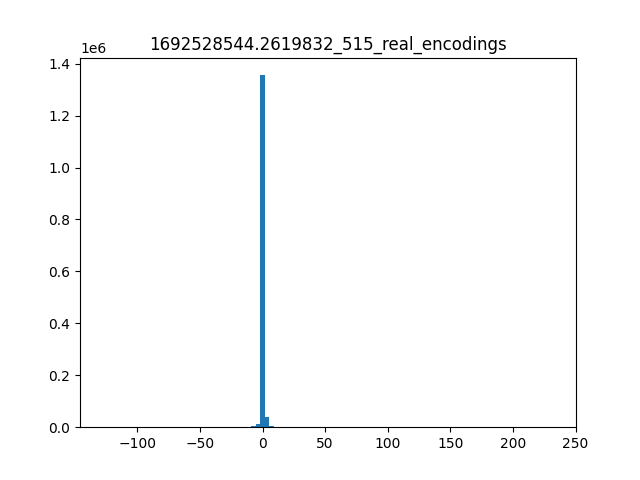
\includegraphics[width=0.6\textwidth]{figures/4.5-results/real_distribution.png}
    \caption{An histogram that represents the latent values created by AudioLDM's \ac{VAE}.}
    \label{fig:original-latents-hist}
\end{figure}

Experience 10 (\ref{sec:exp10}) showed an interesting trend. However, it is worth noting that although the generated spectrograms showed improvement, the generator loss increased while the discriminator loss consistently decreased after a few epochs, as can be seen in Figure~\ref{fig:exp10_loss}. The use of linear layers instead of convolutions proved to be advantageous in generating more robust spectrograms. Further investigation is needed to determine if there are problems with the optimizer.

This last experiment, which used linear layers, produced the most encouraging results and was chosen as the primary study for this dissertation.

\subsection{Results for Future Investigation}

In some experiments, a decline in performance after a few epochs was observed, resulting in losses becoming \ac{NaN}. This is seen in Experiments 8 and 9 (Sections~\ref{sec:exp8}, \ref{sec:exp9}). Further research is required to determine the underlying cause and prevent this occurrence in future experiments.

The impact of elastic network regularization on model performance requires further investigation. Despite the implementation challenges encountered, the initial results suggest that this regularization method has improved and shows potential effectiveness.

In addition, the issue of the continuously increasing generator loss in the last experiment requires further investigation in the future.

\subsection{Interpretation of Results}

The study's findings did not meet the expectations set forth in the thesis as the generated sounds are not state-of-the-art for generative models; however, they are encouraging. With sufficient data and time, the model has the potential to generate high-quality sound. This suggests that generative \ac{AI} models, especially \acp{GAN}, have significant capabilities in audio generation.

Furthermore, exploring the model's latent space is seen as a promising strategy for achieving better results. The latent space method is a simpler approach that can potentially yield more favorable outcomes for future models.

The limitations of the small datasets used in this analysis are evident. The bigger one, Clotho, comprised sounds lasting from 15 to 20 seconds, but with 5 seconds removed from each sound, certain sounds were too short to produce satisfactory results.  Additionally, the total sound count in the data set was less than 5,000, which isn't enough to properly train a generative model.

Thus, a significant concern uncovered in this study is the lack of an appropriate dataset. To achieve more precise results, it is critical to have access to comprehensive datasets. Nevertheless, it is imperative to recognize that the process of training models on large data sets involves significant computational resources that may not be readily available.

\subsection{Conclusion}

In summary, the analysis and interpretation of the data show trends and patterns observed in the experiments. The results did not meet initial expectations; however, they show potential for future advances in generative \ac{AI} models for audio synthesis. It is important to note that comparisons with state-of-the-art audio generation models are not discussed in this study due to the unsatisfactory practical results obtained. 
\section{Constraints and Challenges} \label{sec:res-limitations}

This section discusses the major constraints and challenges faced in developing the proposed solution. It also describes the strategies and solutions adopted or proposed to address these issues, and the potential impacts, tradeoffs, and opportunities that result.

\subsection{Hardware Resources}

One of the biggest challenges was the scarcity of hardware resources for training and evaluating these models. Generative models require large amounts of computing power and memory to process high-dimensional data and learn complex patterns. However, such resources are often limited or expensive to access, especially for individual researchers or small teams. This is a significant barrier to achieving state-of-the-art results in audio synthesis, as few companies and labs have the necessary hardware capabilities.

To overcome this challenge, several strategies have been employed to optimize the use of available hardware resources. First, the neurons of the models were parallelized across the available \acp{GPU} (two in the final configuration --- \ac{LIACC} 2). This allowed to distribute the workload and speed up the training process. Second, checkpoints were implemented to save and load the model state at each epoch. This allowed the training to be resumed from where it was stopped in case of interruptions or failures. Third, the audio files were dynamically read and translated into spectrograms during training. This reduced memory consumption and disk space requirements. Fourth, gradient scaling and autocast (mixed precision training) techniques were used. These techniques involve performing some computationally expensive operations in 16-bit, while performing other numerically sensitive operations, such as accumulations, in 32-bit. This improved the performance and accuracy of the models while reducing memory consumption.

By applying these strategies, the models were trained and evaluated more efficiently and effectively. However, it is also recognized that these strategies have some limitations and trade-offs. For example, parallelizing neurons across \acp{GPU} can introduce communication overhead and synchronization issues. Checkpoints may not capture the full state of the model or optimizer. Dynamic data processing can increase pipeline latency and complexity. Mixed-precision training can introduce numerical errors or instability.

It is important to note that the hardware configuration with some computational power (\ac{LIACC} 2) was only available about a month before the submission of this thesis, so most of the work was done with really scarce resources. This means that the results presented in this thesis may not reflect the full potential or optimal performance of the proposed solution, as more experiments and improvements could be done with more hardware resources.

\subsection{Data Quality and Quantity}

Another challenge was the quality and quantity of available data. Generative models require a large amount of high-quality and diverse data to learn the underlying patterns and distributions of the data domain. However, such data is often scarce or difficult to obtain, especially for audio synthesis from textual input. Existing datasets for this task are either too small, focused on a specific domain, or lack descriptive labels. This limits the generalization and robustness of the models, as they may overfit to the training data or fail to capture the variability and richness of natural language and sound.

To mitigate this challenge, some data augmentation techniques were applied to increase the size and diversity of the data. For example, random cropping was used to generate different segments of audio from the same file. This increased the number of samples and introduced some variation in the data. However, it is also recognized that these techniques are not sufficient to solve the problem of data quality and quantity. Data augmentation may not produce realistic or novel samples but may introduce noise or artifacts into the data.

\subsection{Hyperparameter Tuning}

A final challenge was the time required for the hyperparameter tuning of the generative models. Hyperparameters are parameters that are not learned by the model, but are set by the user prior to training. They include learning rate, batch size, number of layers, number of neurons, activation functions, regularization methods, etc. Hyperparameters significantly impact the performance and behavior of the model, as they determine how the model learns from the data and adapts to different situations. However, finding the optimal values for these hyperparameters is often a tedious and time-consuming process involving trial-and-error experiments with different combinations of values.

Due to time constraints and deadlines, there was insufficient time to fine-tune our hyperparameters for these generative models. All models presented in this thesis are vanilla versions with default or arbitrary values for their hyperparameters. This means they may not reach their full potential or optimal performance in audio synthesis from textual input. Therefore, it is suggested that future work should devote more time and effort to the hyperparameter tuning of our generative models using methods such as grid search, random search, Bayesian optimization, etc.

\section{Conclusion}

In this section, the author discusses the major limitations and challenges they faced in developing the proposed solution. The author has also described how they addressed these issues and the possible implications, trade-offs, and opportunities that arose. Despite these challenges and limitations, the author believes that the proposed solution has several strengths and advantages that advance the state of the art in generative \ac{AI} models for audio synthesis.